\documentclass[a4paper, 11pt, twocolumn]{article}

\usepackage[a4paper, total={6.24in, 8.5in}]{geometry}
\usepackage[utf8]{inputenc}
\usepackage{graphicx}
\usepackage{verbatim}
\usepackage{float}
\usepackage{array}
\usepackage{xfrac}
\usepackage{mathpazo}
\usepackage{amsmath}
\usepackage{bm}
\usepackage{multirow}
\usepackage{makecell}
\usepackage{multicol}
\usepackage{sectsty,textcase}
\usepackage{wrapfig,lipsum,booktabs}
\usepackage{enumitem}
\usepackage{hyperref}
\usepackage{makecell}
\usepackage{array}

\bibliographystyle{plain}
\renewcommand{\thesection}{\arabic{section}}
\setlength{\columnsep}{15pt}
\newcommand{\myparagraph}[1]{\paragraph{#1}\mbox{}\\}

\title{FYS-STK3155/4155 Applied Data Analysis and Machine Learning - Project 2: Classification and Regression }

\author{Lotsberg, Bernhard Nornes \\ Nguyen, Anh-Nguyet Lise \and
\url{https://github.com/liseanh/FYS-STK4155-project2/}}
\date{October - November 2019}
\begin{document}
\twocolumn[
  \begin{@twocolumnfalse}
    \maketitle
    \begin{abstract}
		Neural networks are important learning methods used in both classification 
		and regression. In this project we compare a multilayer perceptron neural 
		network with logistic regression in a credit card default payment 
		classification case, and with linear regression of a two-variable scalar 
		function. For classification, we found the neural network to produce 
		results superior to those of the logistic regression, while we for 
		regression found that the neural network is excessively costly in 
		comparison to more standard linear regression methods with respect to 
		performance and tuning. 
	\end{abstract}
  \end{@twocolumnfalse}
]

\section{Introduction}
Classification in statistical analysis is a useful tool, e.g. for predicting
outcomes of various situations or classifying and sorting large amounts of data. 
There are several common methods to achieve classification models, such as 
boosting, logistic regression, $k$-nearest neighbour etc., each with their own 
disadvantages and strengths. 
The aim of this project is  to study classification and regression problems
through our own implementation of logistic regression and a multilayer perceptron
(MLP) in Python. The particular data set we will be studying for classification
has been used in a prior research paper by Yeh, I. C. and Che-hui Lien about
data mining techniques \cite{origarticle}, which we will compare some of our
results with.  The full data set can be downloaded from the 
\href{https://archive.ics.uci.edu/ml/datasets/default+of+credit+card+clients}{UCI Machine
Learning Repository} \cite{UCI}. The data set contains certain features of
credit card clients' default payment from a Taiwanese bank.
For the regression problem we will use the MLP to approximate Franke's function
and compare with results from a prior project where we used ordinary least
squares, ridge and lasso regression to approximate it. \cite{regpaper}.


\section{Data}
\subsection{Classification - Credit card client data}
For the classification part of this project,  we are using credit card payment
data from a Taiwanese bank downloaded from the \href{https://archive.ics.uci.edu/ml/datasets/default+of+credit+card+clients}{UCI Machine Learning Repository}. The
response variable is a binary variable of default payment with Yes = 1, No = 0.
The original data set consists of 30 000 observations, with 6636 amount of
observations with default payments. There are 23 features, cited
from the original paper they are described as \cite{origarticle}:
\begin{itemize}[leftmargin=5mm, itemsep=0pt,  parsep=1pt]
 \item $X1$: Amount of the given credit (NT dollar): it includes both the individual consumer credit and his/her family (supplementary) credit.
\item $X2$: Gender (1 = male; 2 = female).
\item $X3$: Education (1 = graduate school; 2 = university; 3 = high school; 4 = others).
\item $X4$: Marital status (1 = married; 2 = single; 3 = others).
\item $X5$: Age (year).
\item $X6$ - $X11$: History of past payment. We tracked the past monthly payment
records (from April to September, 2005) as follows: $X6$ = the repayment status in
September, 2005; $X7$ = the repayment status in August, 2005; . . .;$X11$ = the
repayment status in April, 2005. The measurement scale for the repayment status
is: -1 = pay duly; 1 = payment delay for one month; 2 = payment delay for two
months; . . .; 8 = payment delay for eight months; 9 = payment delay for nine
months and above.
\item $X12-X17$: Amount of bill statement (NT dollar). $X12$ = amount of bill
statement in September, 2005; $X13$ = amount of bill statement in August, 2005;
. . .; $X17$ = amount of bill statement in April, 2005.
\item $X18-X23$: Amount of previous payment (NT dollar). $X18$ = amount paid in
September, 2005; $X19$ = amount paid in August, 2005; . . .; $X23$ = amount paid in
April, 2005.
\end{itemize}

\subsection{Regression - Franke's function}
For the regression part part of this project we will be performing regression
analysis on Franke's function $g(x,y)$ with added Gaussian noise $\bm{\varepsilon}
\sim N(0,\  \sigma^2) $. Franke's function is given by
\begin{align}
g(x,y) &= \frac{3}{4}\exp{\left(-\frac{(9x-2)^2}{4}   - \frac{(9y-2)^2}{4}\right)} \nonumber\\
 &+\frac{3}{4}\exp{\left(-\frac{(9x+1)^2}{49}- \frac{(9y+1)}{10}\right)} \nonumber\\
 &+\frac{1}{2}\exp{\left(-\frac{(9x-7)^2}{4} - \frac{(9y-3)^2}{4}\right)} \nonumber\\
 &-\frac{1}{5}\exp{\left(-(9x-4)^2 - (9y-7)^2\right) }  \label{eq:Franke}
\end{align} and is defined on $x,\ y \in [0,1]$. The data we are fitting is
given by
$$G(\bm{x}, \bm{y}) = g(\bm{x}, \bm{y}) + \bm{\varepsilon},$$
where $\bm{x},\ \bm{y}$ are vectors of uniformly spaced values from 0 and 1 of
length $n_x$ and $n_y$ respectively. To directly compare with our previous
project, \textit{Project 1: Regression analysis and resampling methods}
\cite{regpaper}, we choose to generate and analyze the data sets \texttt{franke0},
\texttt{franke1}, \texttt{franke2} as configured in Table \ref{tab:franke_dataset}.
To generate the points, we grid over $n_x$ points in $x$-direction and $n_y$ points
in $y$-direction.
In the previous project we used a 4th order two-dimensional polynomial function
to model Franke's function. To get an understanding of the performance of our
regression model using a neural network compared to a more simple regression
method, we will compare the $R^2$ scores of our neural network results with the
best model obtained in our prior work, which was found using the ordinary least
squares (OLS) method for a 4th order two-dimensional polynomial. The $R^2$ scores
from the linear regression can be found in Table \ref{tab:R2_scores} along with
our neural network results. From the previous project we however only had
results from data sets corresponding to \texttt{franke0} and \text{franke1}.
For a more detailed explanation of how the OLS model was obtained, please refer
to our previous project \textit{Project 1: Regression analysis and resampling
methods }\cite{regpaper}.

\begin{table}[H]
	\caption{Table of the configurations for our generated data sets using
	Franke's function given in Equation (\ref{eq:Franke}) with added noise $\bm
	{\varepsilon} \sim N(0,\  \sigma^2) $. $n_x$ and $n_y$ indicate the number
	of points used to produce the grid in their respective directions.}
	\label{tab:franke_dataset}
	\resizebox{\columnwidth}{!}{
	\begin{tabular}{|l|l|l|l|c|} \hline
	Data set &  Data points	&$n_x$ & $n_y$ & $\sigma$ \\ \hline
	\texttt{franke0} & 400 & 20 & 20 & 1.0\\ \hline
	\texttt{franke1	} & 400 & 20 & 20 & 0.10\\ \hline
	\texttt{franke2} & 40 000& 200 & 200 & 0.10 \\ \hline
	\end{tabular}
	}
\end{table}

\subsection{Preprocessing}
As the Franke data set is simulated, it does not require as much preprocessing as
the real-life credit card data set does. Additionally, the credit card data set
contains both categorical and continuous variables, whereas the Franke data set
only contains continuous variables. Due to this, we will start by discussing the
inital steps in the preprocessing of the credit card data.

We first removed feature outliers in the credit data set by looking at the supposed
discrete values of $X2-X4$ and $X6-X11$. However, though in the original paper
they stated that $X6-X11$ $\in\{-1,\ 1,\ 2,\ 3,\dots,\ 9\}$, the majority of
the samples contained the values 0 and 2, which were undefined. Removing these
would have reduced the data set down to only approximately four thousand data
points, so we have opted to keep them in our analysis as unexplained variables
and ended up with a data set of 29603 points, 6606 of which were default payments.

To ensure that the categorical variables $X2$-$X4$ in the credit card set were
considered equal by the classifiers, we incorporated the use of dummy variables
and one-hot encoded the variables.

We use \texttt{Scikit-learn's}\cite{sklearn_api} library to split both data sets
into test and training sets, and to scale and center the data.
For both data sets we used $1/3$rd of the total data as testing data
and the remaining $2/3$rds as training. To center the data, the means of the
continuous variables in the training set were subtracted from both the training
and the test sets. Each continuous variable in the training and test sets was
scaled with respect to its standard deviation in the training set.

Before scaling the credit card data set, we first opted to upsample the number of
default payment samples in the training set by using
\resizebox{!}{6.38pt}{\texttt{imblearn.over\_sampling.RandomOverSampler}}
from the library \texttt{imbalanced-learn}, which randomly duplicates the default
payment samples, until there was an equal amount of default payment samples as
non-default samples. This was done to improve the model prediction. Note that we
did not upsample the amount of defaults in the test set.


\section{Learning methods}
\subsection{Logistic Regression (LR)}
Logistic regression (LR)  is a statistical model that can be used to predict a
binary dependent variable, which in our project will be one of the methods used
for binary classification of the credit card default/non-default payments. LR
outputs the probability of a sample to be in either 1 (default) or non-default (0),
with the probability being given by the logit (Sigmoid) function, such that
\begin{align}
p(y=1 | \bm{X}, \bm{\beta}) &= \frac{1}{1 + e^{-\bm{X} \bm{\beta}}} =
\frac{e^{\bm{X} \bm{\beta}}}{e^{\bm{X} \bm{\beta}}+1},\\
p(y\neq1 | \bm{X}, \bm{\beta}) &= 1 - p(y=1 | \bm{X}, \bm{\beta})\ .
\label{eq:LR_probability}
\end{align}
Here $\bm{X}$ is the feature matrix, and $\bm{\beta}$ is a vector containing the weights
assigned to each feature in $\bm{X}$.  The cost function most commonly used in this
case is called the cross entropy, which is the negative log-likelihood of a prediction
being in the dataset and is given by
\begin{align}
\mathcal{C_\text{ LR}}(\bm{\beta}) =& -\sum_{i=0}^{n-1} \left[\  y_i\log p(y_i|x_i, \bm{\beta}) \right. \nonumber\\
 &\left.+ (1-y_i)\log(1-p(y_i|x_i,\bm{\beta})    \right]
\end{align}


To optimize the cost function, we find the optimal weights $\bm{\beta}$ by
solving $\text{argmin}_{\bm{\beta}}$. Similarly to for LASSO regression, which
we used in our previous project, this has no analytical solution and must be
estimated using numerical methods, e.g. gradient descent \cite{regpaper}. This
along with its stochastic sibling is described in section \ref{SGD}.

When using the model for prediction, $\hat{y}=p(X)\in [0, 1]$, where we say
that outcome 0 is predicted if $\hat{y}< 0.5$ and outcome 1 else.

In this project we will use LR on the Taiwanese credit card data to try to predict
default ($y=1$) or non-default ($y=0$) payment and evaluate the model's predictive
accuracy in this particular classification problem.

\subsection{Neural Networks (NN)}

An artificial neural network (NN) is a computational model consisting of
interconnected nodes. The interconnected nodes aim to emulate a simplified
biological neural network and neuronal firing in a brain, and are therefore
also commonly referred to as neurons.  The node performs a weighted sum of its
inputs that is subsequently passed through a mathematical function to determine
its output. This mathematical function is called an activation function $f(z)$,
and should emulate neuronal firing.

There is a wide variety of different neural networks. Commonly, they consist of
layers of nodes separated into the input layer and output layer, and may also
contain one or more in-between layers called hidden layers. One such NN is the
multilayer perceptron (MLP), which is what we will be using in this project for
both classification and regression.
\subsection{Multilayer perceptron (MLP)}

\subsubsection{Feed-forward  }
The multilayer perceptron is a feed-forward neural network (FFNN), which means
that the information flows forward only, starting from the input layer and to
the output layer. Additionally, if each of the nodes in a layer are connected to
all of the nodes in the succeeding layer, the network is fully connected. The
inputs of the node are the weighted outputs of the nodes from the preceding
layer, in addition to a bias term that can control whether or not the neuron
fires if all the inputs are zero \cite{ML_algo}. The weighted sum of the inputs
of each node is called the activation.

\subsubsection*{Mathematical algorithm} \myparagraph{Input layer}
Starting with the input layer, which is the first layer in the MLP, the
activation is calculated using the input coordinates $x_j$,
\begin{equation}
z_i^1 = \sum^{M_1}_{j=1}w_{ij}^1x_j + b_i^1,
\end{equation}
where the superscript 1 indicates the first layer, $M_1$ is the number of inputs
to the $i$th node in the first layer, $b_i$ is the bias and $w_{ij}$ represents
the weights.

The output of the nodes in the input layer is determined by the activation
function $f(z)$,
\begin{equation}
f(z_i^1) = f \left( \sum^{M_1}_{j=1}w_{ij}^1x_j + b_i^1 \right)
\end{equation}
\myparagraph{Hidden layers and output layer}
Similarly for the subsequent layers; the hidden layers and the output layer, the
activation of the $j$th neuron of layer $l$ is defined as
\begin{equation}
z_j^l = \sum_{i=1}^{M_{l-1}} w_{ij}^la_j^{l-1} + b_j^l,
\end{equation}
where $b_j^l$ and $w_{ij}^l$ are the biases and weights at layer $l$, ${M_{l-1}}$
is the number of nodes at layer $l-1$ and $a_j^{l-1}=f(z_j^{l-1}) $.
The output of each node is then decided by passing the activation through the
activation function,
\begin{equation}
 f(z_j^l) =f \left(     \sum_{i=1}^{M_{l-1}} w_{ij}^la_j^{l-1} + b_j^l \right)
\end{equation}
This is nearly identical to the method for the input layer, except that the
inputs of these layers are the outputs from the previous layer.

\subsubsection{Backpropagation} \label{subsub:backpropagation}
In order for the NN to learn, the weights and biases are initialized with values
that we will discuss shortly. The weights and biases are then optimalized to
minimize the cost function through a process called backpropagation, where we
iterate backwards from the last layer to the first hidden layer. Another feed-forward process is initiated  from the input layer to the output layer with the new
biases and weights. If the cost function is not yet sufficiently minimized, then
backpropagation is performed again. This process is repeated until the cost
function is optimalized.

\myparagraph{Mathematical algorithm}
To calculate the optimal biases and weights for the problem, we initialize the
gradients of the cost function $\mathcal{C}$ with respect to the  weights $W$
and biases $b$ at the output  layer $l=L$ 	and the output error $\delta_L$ as
\begin{flalign}
&\frac{\partial  \mathcal{C}}{\partial w^L_{jk}} = \delta^L_j a_k^{L-1},
\label{eq:dC/dw_L}\\
&\frac{\partial  \mathcal{C}}{\partial b^L_j} = \delta^L_j,\\
&\delta_j^L= f'(z_j^L)\frac{\partial \mathcal{C}}{\partial a_j^L},
\label{eq:delta_j^L}
\end{flalign}
before propagating backwards through the hidden layers using the general equations
\begin{flalign}
&\frac{\partial  \mathcal{C}}{\partial w^l_{jk}} = \delta^l_j a_k^{l-1},
\label{eq:dC/dw_l} \\
&\frac{\partial  \mathcal{C}}{\partial b^l_j} = \delta^l_j,\\
&\delta_j^l= \sum_k \delta_k^{l+1}w_{kj}^{l+1}f'(z_j^l). \label{eq:delta_j^ l}
\end{flalign}
The full derivation of these equations can be found in \textit{Neural networks,
from the simple perceptron to deep learning} by Morthen Hjorth-Jensen \cite{morten_NN}.

\subsubsection{Choosing activation function}
There are certain properties that an activation function $f(z)$ should possess
\cite{ML_algo}:
\begin{enumerate}
\item $f(z)$ should be differentiable (continuous). \label{item:differentiable_f}
\item $f(z)$ should be non-constant and reach saturation at both ends of the range.
\item $f(z)$ should change quickly between the saturation values  at the middle
of the range.
\end{enumerate}
It is clear  from Equation (\ref{eq:delta_j^ l}) in the backpropagation algorithm
that the activation function $f(z)$ should be differentiable, while the remaining
properties are mainly related to the emulation of firing of neurons in a brain.

There are several functions that meet these requirements. Historically, the
sigmoid function has been a popular choice of activation function until recently.
To compare our results with the original paper from 2009 by I-Cheng Yeh and
Che-hui Lien \cite{origarticle}, we have chosen to use the sigmoid function in
our implementation of the MLP, as it is likely the same function they used. The
function is given by
\begin{equation}
	f(z) = \frac{1}{1+e^{-z}}\ .
\end{equation}
Its gradient is given by
\begin{equation}
	\label{eq:df/dz}
	\frac{\partial f}{\partial z} = \frac{e^{-z}}{(1+e^{-z})^2}.
\end{equation}
However, there are cases where we do not want a sigmoidal output activation
function, such as for regression problems where the outputs should be from a
continuous range instead of binary. Instead of a sigmoidal activation function
for the regression case at output layer $l=L$, we implement a linear activation
function, such that
\begin{equation}
f(z_j^L)=z_j^L= \sum_{i=1}^{M_{L-1}} w_{ij}^L a_j^{L-1} + b_j^L.
\end{equation}
For our binary classification case, we keep the sigmoid function as the output
activation function.
\subsubsection{Choosing cost function}
Looking at the equations for backpropagation, it is clear that the chosen cost
function $\mathcal{C}$ should be differentiable as well.
Additionally, the cost function should be chosen with the desired functionality
in mind, i.e. the cost functions for regression and classification should be different.

For the classification part of this project we have chosen to use the logistic
loss as cost function, which is the negative log-likelihood,
\begin{align}
\mathcal{C_\text{ NN}^\text{ C}}&(\bm{W}, \bm{b}) = -\sum_{i=0}^{n-1}
\left[\  a_i^l\log p\left(a_i^l|z_i^l,\ \bm{ W,\ b} \right) \right.  \\
&   \left. + (1-a_i^l)\log \left(1-p(a_i^l|z_i^l,\ \bm{ W,\ b} )\right) \right],
\nonumber
\end{align}
with $a_i^l=f(z_i^l)$ as before. The gradient at the last layer is
\begin{align}
\frac{ \partial C_\text{ NN}^\text{ C}}  {\partial a_i^L} =
a_i^L-t_i, \label{eq:dC/da_NN^C}
\end{align}
where $t_i$ is the target.\\

For the regression part we will use the cost function
\begin{equation}
\mathcal{C}_\text{ NN}^\text{ R} = \frac{1}{2}\sum_{i=0}^{n-1}(t_i-a_i^l)^2.
\end{equation}
The gradient in the last layer is given by
\begin{equation}
	\frac{\partial \mathcal{C}_\text{ NN}^\text{ R}}{\partial a_i^L}=t_i -a_i^L\ .
	\label{eq:dC/da_NN^R}
\end{equation}

The gradients in Equation (\ref{eq:dC/da_NN^C}) and (\ref{eq:dC/da_NN^R}) can then be inserted into Equation (\ref{eq:delta_j^ l}) in the backpropagation algorithm.
\subsubsection{Initialising  the weights and biases}
The biases can be initialized to zero, but we have chosen an initial value of 0.01
to ensure that all of the neurons have some initial output. Initializing the
weights to zero, however, will result in all neurons outputting the same value.
Instead, the  weights are initialized with values drawn from a uniform distribution
such that $w_{kj}\in (-1/\sqrt{n}, \ 1/\sqrt{n})$, where $n$ is the amount of
nodes in the input layer,  to ensure uniform learning \cite{ML_algo}.

\subsubsection{Regularization}
As neural networks often have large amounts of parameters, they are considered
very high variance low bias estimators. This means they are very prone to
overfitting. To counteract this, we introduce regularization using the $L_2$
penalty on the weights similarily to Ridge regression. Mathematically, this means
adding the regularized cost function becomes
\begin{equation}
  \mathcal{C}_{\text{Regularized}} = \mathcal{C}_\text{ NN}^{C/R} + \lambda ||\bm{W}||_2^2
  \label{Regularized cost}
\end{equation}
and its derivative becomes
\begin{equation}
  \frac{ \partial C}  {\partial \bm{W}}_\text{Regularized}
  = \frac{ \partial C_\text{ NN}^\text{ C/R}}  {\partial \bm{W}} + \lambda \bm{W}.
\end{equation}
Here $\lambda$ is a hyperparameter we need to tune.

\subsection{Stochastic Gradient Descent (SGD)}
\label{SGD}
It is clear that in order to find the best possible fit, we need to optimize the
cost function $\mathcal{C}$ by finding its minimum. A common method to achieve
this is the gradient descent (GD) method, in which the parameters $\theta$ are
iteratively adjusted in the direction of the largest negative value of the
gradient for a given number of epochs or until it reaches a given tolerance.
Mathematically, this is expressed as
\begin{equation}
\theta_{i+1} = \theta_i -\eta \nabla \mathcal{C}(\theta_i),
\end{equation}
where $\eta$ is the learning rate, which is a hyperparameter that controls the
step length and by extension the convergence time. For smaller values of $\eta$,
the method will take longer to converge or might not converge at all within the
maximum number of epochs. For larger values of $\eta$, the method might be unstable or
pass the minimum altogether and diverge. The parameter $\theta$ is $\beta$ in
the LR case, and the weights $W$ and biases $b$ in the MLP case.
Our definition of convergence is when the cost function does not change by more
than a factor 0.01 for ten epochs.

However, calculating the gradient on the entire data set can be computationally
expensive and inefficient for large amounts of data. Additionally, there is a high
possibility of a local minimum being misinterpreted as a global minimum by the
algorithm. To alleviate these problems, we can use stochastic gradient descent
(SGD) with minibatches.  A minibatch is a subset of the data, on which we can
perform GD. By using stochasticity to perform gradient descent on randomly chosen
minibatches of size $M$, we have a more efficient way to approximate the gradient
of the total data set as it might not need to use the entire set. Additionally,
the stochasticity reduces the possibility of getting stuck in a local minimum.

\subsection{Tuning hyperparameters}
\label{subsec:tuning_hyperparameters}
Hyperparameters are not estimated when fitting a model, and must instead be
found by other means. A naive approach when you have few hyperparameters could
be to find them manually by trial and error. A slightly better approach is to
grid over your hyperparameter space. However, this can be very computationally
expensive. Studies indicate that a random search is preferable, as it is less
systematic than a grid search, and thus more statistically likely to find better
hyperparameters  \cite{bergstra2012random}. For each trial parameter, one evaluates
the model on the training data, preferably either splitting some of
the training data into validation data or using cross validation to avoid overfitting.
The final best model is then evaluated using the test data.

For non-penalized logistic regression with stochastic gradient descent,
the two hyperparameters are learning rate and batch size. We have chosen to use
a batch size of 200, inspired by the default value of Scikit-Learn. If we had
more time or more powerful hardware, we would ideally also try different batch sizes.
The learning rate is found using a randomized search with cross validation.

Neural networks contain many hyperparameters. The amount of layers, nodes in each
layer, batch size, learning rate and penalization should all ideally be tested.
As with LR, we have chosen to use a constant batch size of 200. For the layers
and nodes, we have chosen to limit ourself to two hidden layers with many nodes.
A neural network with a single hidden layer with a large amount of nodes is already
sufficient enough to be considered a universal approximator. With two hidden layers,
the amount of nodes needed is reduced \cite{ML_algo}, making a two hidden layer
neural network sufficient for most cases. For both datasets analyzed, our first
hidden layer has 100 nodes, the second has 50. This leaves the learning rate and
the regularization parameter which are found using randomized search.

To perform the parameter search we use the \texttt{RandomizedSearchCV} class provided
by \texttt{Scikit-Learn} \cite{sklearn_api} on 100 samples of hyperparameters,
with 5-fold cross validation to evaluate each sample. The maximum number of epochs
is set to 300 for all models. Our evaluation methods are explained in the next section.

\section{Model evaluation}
\subsection{Regression}
To evaluate the performance of our regression model, we consider the $R^2$ score,
given by
\begin{equation}
	R^2(\bm{y}, \bm{\hat{y}}) = 1 - \frac{\sum_{i=0}^{n - 1} (y_i -
	\hat{y}_i)^2}{\sum_{i=0}^{n - 1} (y_i - \bar{y})^2},
    \label{eq:R2}
\end{equation}
where $\bm{y}$ is the given data, $\bm{\hat{y}}$ is the model and ${\bar{y}}$ is
the mean value of $\bm{y}$. The $R^2$ score evaluates how well your model
$\bm{\hat{y}}$ fits the true values $\hat{y}$, with a value of 1 indicating a
perfect fit. An $R^2$ score of 0 indicates that the model is as good of an
estimator as the mean value ${\bar{y}}$, and a lower value means that the mean
value is a better estimator than the model.


\subsection{Classification}
\label{Classification}
To evaluate the performance of our classification model, we consider the accuracy
score, given by
\begin{equation}
\label{eq:accuracy}
\text{accuracy}=\frac{\sum_{i=1}^nI(t_i=y_i)}{n},
\end{equation}
where $t_i$ is the target, $y_i$ is the model output, $n$ is the number of
samples and $I$ is the indicator function,
\[
I = \begin{cases}
1, & t_i = y_i\\
0, & t_i \neq y_i
\end{cases} .
\]
The error rate used in the original article \cite{origarticle} is then defined as
\begin{equation}
\text{error} = 1 - \text{accuracy}.
\label{error}
\end{equation}

For the data used in this project, this is not a very good metric however. This is
because even a model that predicts 0 for all cases would get an accuracy score of
nearly 0.8 due to the large ratio of non-default payments to default payments in
the credit card data set. The need for a better model evaluation is clear, and
we employ the same technique as in the original article by I-Cheng Yeh and Che-hui
Lien, which was the area ratio \cite{origarticle} between the baseline and our
model in a cumulative gains plot divided by the area between the theoretically
best model and the baseline. To generate cumulative gains plots, we used the
Python library \texttt{Scikit-Plot}'s function \texttt{plot\_cumulative\_gain}.
An area ratio of 1 would simply be the theoretically most optimal fit, whereas
lower ratios indicate lower predictive ability of the model.

\section{Results}
Figure \ref{fig:logreg_eta_accuracy} shows the accuracy score for LR on the credit
card training and validation data set for 100 different values of the learning
rate $\eta$ found using randomized search. Looking at the figure, we observe
that the accuracy  score drops significantly for learning rates at the higher
and lower values of the range. The learning rate value that maximizes the
accuracy score is considered the best value and is shown in Table
\ref{tab:hyperparameters}.

\begin{figure}[H]
	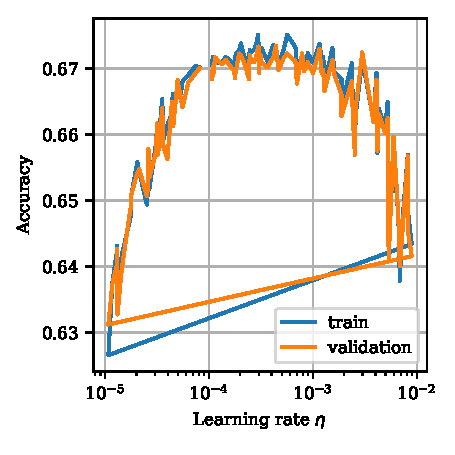
\includegraphics[scale=1]{figures/logreg_learning_rate_accuracy.pdf}
	\caption{Accuracy score of validation set of the credit data using  logistic
	regression for various values of the shrinkage parameter
	chosen using randomized search.}
	\label{fig:logreg_eta_accuracy}
\end{figure}

Similarly, Figure \ref{fig:nn_eta_lambda_credit_accuracy} shows the accuracy
score for the MLP classifier used on the credit card data set for 100 different
combinations of values for the learning rate $\eta$ and the shrinkage parameter 
$\lambda$ configured using random search. The figure shows that most of the
combinations of our learning and shrinkage parameters in our chosen range give
an accuracy score between approximately 0.65-0.70, with the exception of a few
outliers. Generally, it seems like accuracy scores improve with smaller learning
rates within our chosen range. The effect of the choice of shrinkage parameter
is not as conclusive, although it seems like the score is lower when the
shrinkage parameter is of orders larger than $10^{-2}$. The combination of
learning rate and shrinkage parameter that gives the highest accuracy score is
considered the most optimal of our combinations, and is also shown in Table
\ref{tab:hyperparameters}.


\begin{figure}[H]
	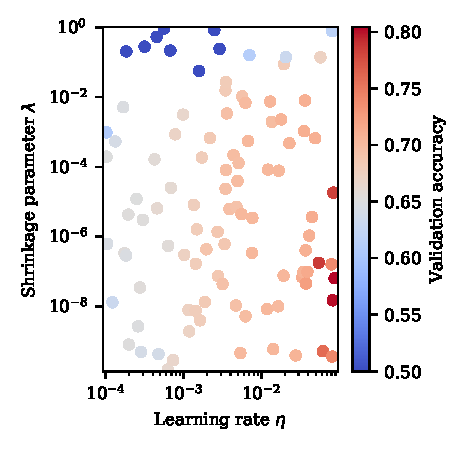
\includegraphics[scale=1]{figures/nn_learning_rate_lambda_accuracy_credit.pdf}
	\caption{Accuracy score of validation set of the credit card data using the
	multilayer perceptron classifier on the credit card data for various shrinkage
	parameters and learning rates chosen using randomized search.}
	\label{fig:nn_eta_lambda_credit_accuracy}
\end{figure}

Figure \ref{fig:nn_eta_lambda_r2_400_1.0}, \ref{fig:nn_eta_lambda_r2_400_0.1} and
\ref{fig:nn_eta_lambda_r2_40000_0.1} show the validation $R^2$ scores for the MLP
regressor on the \texttt{franke0}, \texttt{franke1} and \texttt{franke2} data
sets, respectively. For a reminder of the differences between these data sets,
please refer to Table \ref{tab:franke_dataset}. As for the classification methods,
the models were evaluated for 100 different combinations of learning rate and
shrinkage parameter values.

\noindent For \texttt{franke0} in Figure
\ref{fig:nn_eta_lambda_r2_400_1.0}, the $R^2$ score is the lowest for the higher
values of the learning rate in the chosen range at around order $10^{-3}-10^{-2}$
and the highest between approximately $10^{-4}-10^{-3}$. The shrinkage parameter
values in our range do not seem to have a large effect on the $R^2$ score of the
model.

\noindent For \texttt{franke1} in Figure \ref{fig:nn_eta_lambda_r2_400_0.1}, the
learning rates of order around $10^{-2}$ seem to result in the lowest $R^2$
scores, as well as a small amount of outliers at learning rates of order $10^{-5}$,   whereas the highest $R^2$ scores seem to be at around learning rates of order
$10^{-4}$. Shrinkage parameters of order $10^{-2}$ and higher result in a lower
$R^2$ score.

\noindent For \texttt{franke2} in Figure \ref{fig:nn_eta_lambda_r2_40000_0.1},
there is not a large difference in $R^2$ scores between learning rates of order
$10^{-5}-10^{-3}$, where they are the highest. They are lowest for larger values
of learning rates. Additionally, the shrinkage parameters of order $10^{-3}$ or
larger drastically reduce the $R^2$ scores, while smaller values seem to result
in better scores.

\noindent The most optimal models for the regression case were the ones that
maximized the $R^2$ scores. The corresponding shrinkage parameter and learning
rate values can be found in Table \ref{tab:hyperparameters}.


\begin{figure}[H]
	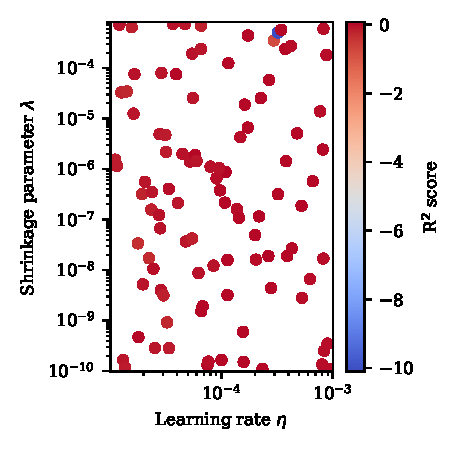
\includegraphics[scale=1]{{figures/nn_learning_rate_lambda_r2_franke_20_20_1.0}.pdf}
	\caption{$R^2$ score of validation set on the \texttt{franke0} data set using
	the multilayer perceptron regressor for various shrinkage parameters and
	learning rates chosen using randomized search.}
	\label{fig:nn_eta_lambda_r2_400_1.0}
\end{figure}


\begin{figure}[H]
	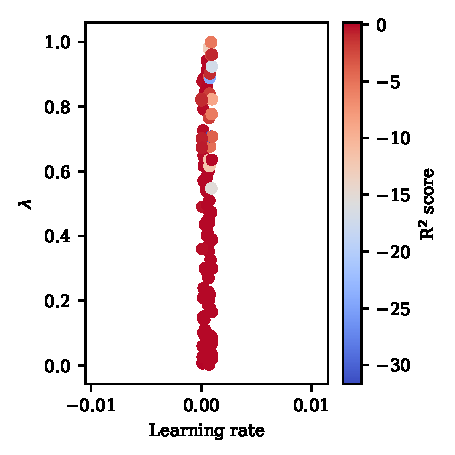
\includegraphics[scale=1]{{figures/nn_learning_rate_lambda_r2_franke_20_20_0.1}.pdf}
	\caption{$R^2$ score of validation set on the \texttt{franke1} data set using
	the multilayer perceptron regressor for various shrinkage parameters and
	learning rates chosen using randomized search.}
	\label{fig:nn_eta_lambda_r2_400_0.1}
\end{figure}

\begin{figure}[H]
	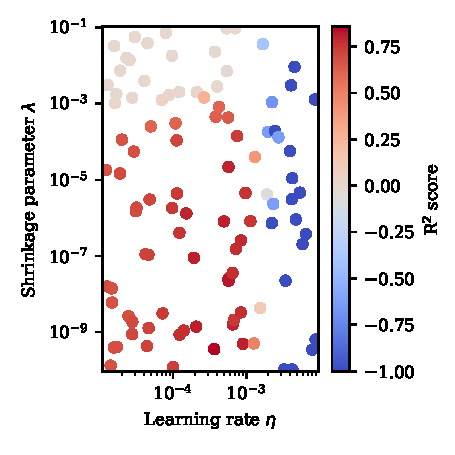
\includegraphics[scale=1]{{figures/nn_learning_rate_lambda_r2_franke_200_200_0.1}.pdf}
	\caption{$R^2$ score of validation set on the \texttt{franke2} data set using
	the multilayer perceptron regressor for various shrinkage parameters and
	learning rates chosen using randomized search.}
	\label{fig:nn_eta_lambda_r2_40000_0.1}
\end{figure}



\begin{table}[H]
	\caption{Table of the best hyperparameters values for shrinkage $\lambda$ and
	learning rate $\eta$ for the logistic regression (LR) and neural network (NN)
	models. The parameters were found using 5-fold cross validation. The minibatch
	size was kept constant at $M=200$. All the results have been modelled using
	these values.}
	\label{tab:hyperparameters}
  {\setlength{\extrarowheight}{2pt}
		\resizebox{\columnwidth}{!}{
	\begin{tabular}{|l|l|l|}
	  \hline
	  Model & Shrinkage $\lambda$ & Learning rate $\eta$ \\ \hline
	  LR credit data & N/A & $4.4 \cdot 10^{-4}$ \\ \hline
	  NN credit data & $6.9 \cdot 10^{-7}$ & $7.7 \cdot 10^{-2}$ \\ \hline
	  NN \texttt{franke0} & $4.1\cdot 10^{-6}$ & $9.1\cdot 10^{-5}$ \\ \hline
	  NN \texttt{franke1} & $6.4\cdot 10^{-8}$ & $1.5 \cdot 10^{-4}$\\ \hline
	  NN \texttt{franke2} & $3.6\cdot 10^{-10}$ & $3.7 \cdot 10^{-4}$\\ \hline
	\end{tabular}
	}}
  \end{table}



\subsection{Classification}
Figure \ref{fig:logreg_gain} shows the cumulative gains plot for the LR. From
the figure, we can see that our LR model performs worse when predicting
non-default outcomes than default. Both area ratios can be found in Table
\ref{tab:area_ratios}.


Figure \ref{fig:nn_gain} shows the cumulative gains plot for the MLP classifier.
From the figure, we can see that similarly to for the LR model, the MLP
classifier model's predictive abilities are better for default outcomes than for
non-default. Both area ratios can be found in \ref{tab:area_ratios}.

From Table \ref{tab:area_ratios} containing the area ratios for LR and MLP, we
see that the MLP network has a lower error rate than LR, in addition to having
higher area ratios for both default and non-default outcomes.

\begin{figure}[H]
	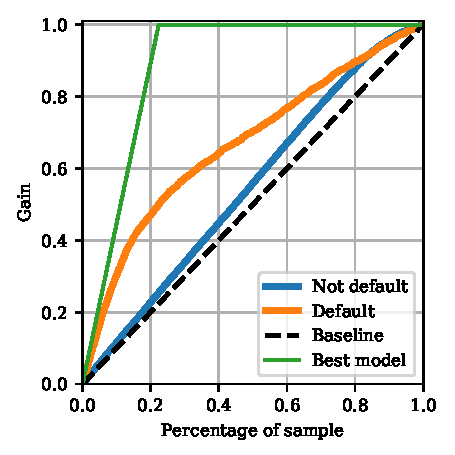
\includegraphics[scale=1]{figures/cumulative_gain_logreg.pdf}
	\caption{Cumulative gains plot for the logistic regression model fit on the
	credit card data.}
	\label{fig:logreg_gain}
\end{figure}




\begin{figure}[H]
	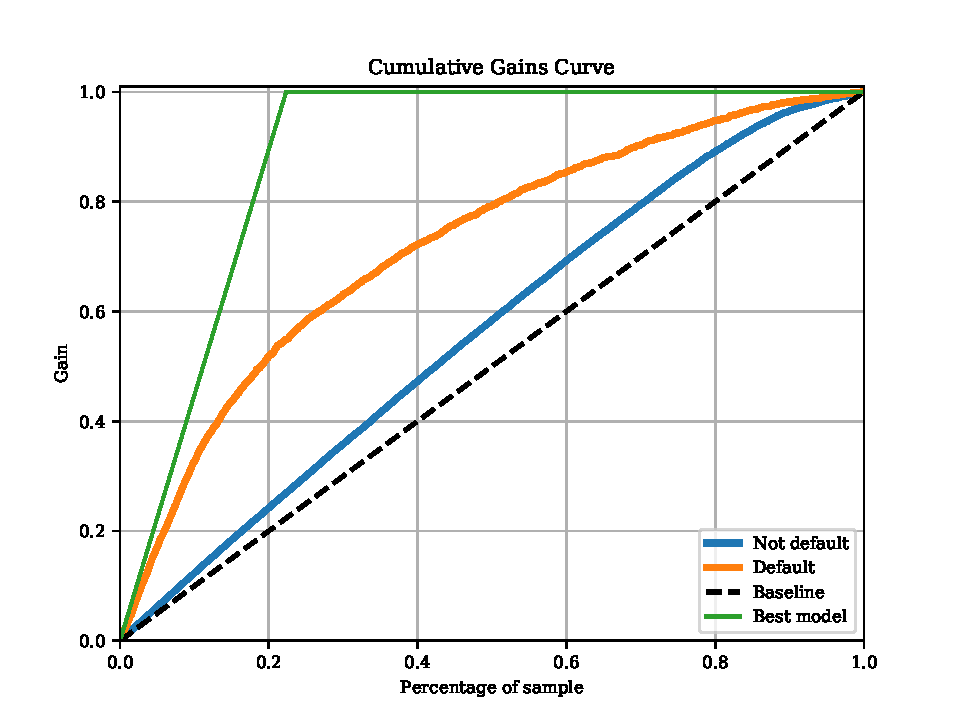
\includegraphics[scale=1]{figures/cumulative_gain_NN.pdf}
	\caption{Cumulative gains plot for the multilayer perceptron model fit on
	the credit card data.}
	\label{fig:nn_gain}
\end{figure}



\begin{table}[H]
	\caption{Table of the error rates and area ratios for classification of the
	credit card data using our logistic regression (LR) and multilayer
	perceptron (MLP) neural network (NN). The results from the original paper are
	also included, indicated with subscript O in the table \cite{origarticle}. }
	\label{tab:area_ratios}
	\resizebox{\columnwidth}{!}{
 	\begin{tabular}{|l|l|l|l|}
    \hline
 	   Method & \makecell[l]{Error \\rate} & \makecell[l]{Area ratio \\default} & \makecell[l]{Area ratio \\non-default} \\ 			\hline
    		LR 			  & 0.31 & 0.43 & 0.12 \\ \hline
			NN 			  & 0.22 & 0.55 & 0.16 \\ \hline
			LR$_\text{O}$ & 0.18 & 0.44 & N/A\\ \hline
			NN$_\text{O}$ & 0.17 & 0.54 & N/A \\ \hline
    	\end{tabular}
	}
\end{table}

\subsection{Regression}
Table \ref{tab:R2_scores} shows the $R^2$ scores for the \texttt{franke0},
\texttt{franke1} and \texttt{franke2} data sets using the MLP regressor in
addition to the scores found using the OLS model. For the \texttt{franke0} set,
the MLP and OLS seem to perform similarly, with scores lying in a small interval
around zero. For \texttt{franke1} the score for OLS is significantly higher, while
the OLS model for \texttt{franke1} and the MLP model for \texttt{franke2} show
similar performances. The consistency of the $R^2$ score across training and test
sets is better for the MLP model in the cases of \texttt{franke1} and
\texttt{franke2}.

Figure \ref{fig:3dplot_400_1.0}, \ref{fig:3dplot_400_0.1} and
\ref{fig:nn_eta_lambda_r2_40000_0.1} show the MLP models for the
\texttt{franke0}, \texttt{franke1} and \texttt{franke2} data sets plotted with
the true values.

\begin{table}[H]
	\caption{Table of R2 scores for our neural network (NN) regression models on
	the three Franke data sets and the ordinary least squares (OLS) model from our
	previous study \cite{regpaper}. }
	\label{tab:R2_scores}
	\resizebox{\columnwidth}{!}{
 	\begin{tabular}{|l|r|r|r|r|}
    \hline
 	     {} &$R^2$  & \texttt{franke0} & \texttt{franke1} &	\texttt{franke2} \\	\hline
    	 \multirow{2}{*}{NN}  &Train   & 0.0052  & 0.59 & 0.84 \\ \cline{2-5}
    		 				  &Test    & - 0.057 & 0.59 & 0.83 \\ \hline
    \multirow{2}{*}{OLS}      &Train   & 0.024   & 0.87	& N/A \\ \cline{2-5}
    		 				  & Test   & - 0.040 & 0.82 & N/A\\ \hline
    	\end{tabular}
	}
\end{table}
\begin{figure*}
	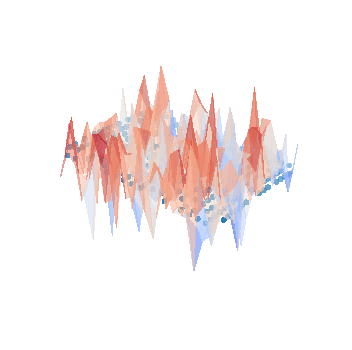
\includegraphics[width=\columnwidth]{{figures/3dplot_train_20_20_1.0}.pdf}
	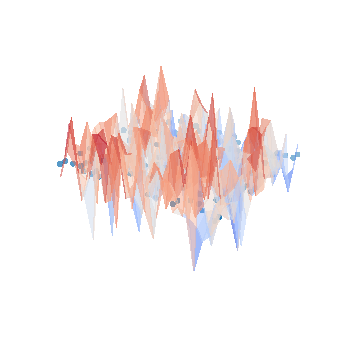
\includegraphics[width=\columnwidth]{{figures/3dplot_test_20_20_1.0}.pdf}
	\caption{3D plot of the Franke function with added noise $\sim\mathcal{N}(0,
	\sigma^2)$ with $\sigma=1.0$. The dotted markers represent the regression
	model found using MLP. The left plot shows the model fitted on the training
	set, the right shows the model fitted on the test set. The total data set
	consist of 400 points, using two thirds $(\sfrac{2}{3})$ as the training set
	and the remaining points $(\sfrac{1}{3})$ as the test set. }
	\label{fig:3dplot_400_1.0}
\end{figure*}

\begin{figure*}
	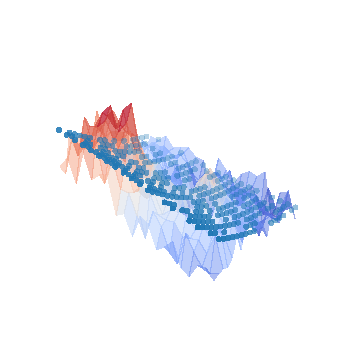
\includegraphics[width=\columnwidth]{{figures/3dplot_train_20_20_0.1}.pdf}
	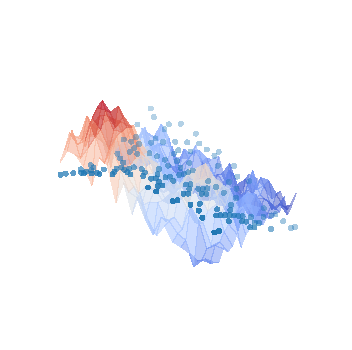
\includegraphics[width=\columnwidth]{{figures/3dplot_test_20_20_0.1}.pdf}
	\caption{3D plot of the Franke function with added noise $\sim\mathcal{N}(0,
	\sigma^2)$ with $\sigma=0.1$. The dotted markers represent the regression
	model found using MLP. The left plot shows the model fitted on the
	training set, the right shows the model fitted on the test set. The total
	data set consist of 400 points, using two thirds $(\sfrac{2}{3})$ as the
	training set and the remaining points $(\sfrac{1}{3})$ as the test set. }
	\label{fig:3dplot_400_0.1}
\end{figure*}

\begin{figure*}
	\includegraphics[width=\columnwidth]{{figures/3dplot_train_200_200_0.1}.pdf}
	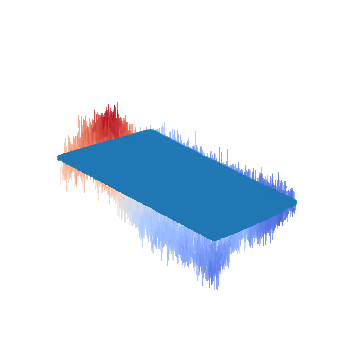
\includegraphics[width=\columnwidth]{{figures/3dplot_test_200_200_0.1}.pdf}
	\caption{3D plot of the Franke function with added noise $\sim\mathcal{N}(0,
	\sigma^2)$ with $\sigma=0.1$. The dotted markers represent the regression
	model found using MLP. The left shows the model fitted on the training set,
	the right shows the model fitted on the test set. The total data set consist
	of 40 000 points, using two thirds $(\sfrac{2}{3})$ as the training set and
	the remaining points $(\sfrac{1}{3})$ as the test set. }
	\label{fig:3dplot_40000_0.1}
\end{figure*}



\section{Discussion}

\subsection{Classification}
From Table \ref{tab:hyperparameters}, we see that the learning rate $\eta$ for
LR and MLP in the classification case differ by two orders of magnitude. This is
most likely because the MLP is a more advanced model, and therefore the parameter
space has a more easily achievable minimum, although the parameter space is much
higher dimensionally than for LR.


The area ratios in Table \ref{tab:area_ratios} along with Figure
\ref{fig:logreg_gain} and \ref{fig:nn_gain} align closely
with the results from the original paper \cite{origarticle}, with the MLP being
noticeably better at predicting the default of a credit card user than LR, with
area ratios for the positive outcome being $0.55$ and $0.43$ respectively.
While both models can predict the positive outcome with modest success, they are
not suited for predicting the negative outcome within any kind of satisfactory
margin. In spite of this, in the context of banking, it is better to refuse a 
loan that would likely be repaid than to lend to a client that might not be able 
to repay the debt. With this we argue that it is beneficial to implement a MLP 
classifier in this case in spite of the extra computational cost and the extra 
hyperparameters.

Comparing our results to the ones in the original paper in the Table 
\ref{tab:area_ratios}, we see that we were not able to achieve as good error rates 
as the original authors, whilst our area ratio for the default NN payment is only 
slightly better. It is not clear why, as the paper only explains in general terms
which methods were implemented without detailing tuning of hyperparameters and 
initializations of e.g. weights and biases. 

\subsection{Regression}
Looking at the shrinkage parameters for the regression models in Table
\ref{tab:hyperparameters}, the shrinkage parameter seems to decrease as the
signal to noise ratio increases. For $\texttt{franke0}$, the data set is quite
noisy with the standard deviation of the added noise at $\sigma=1.0$ and a
shrinkage parameter of $\lambda=4.1\cdot 10^{-6}$. However, taking Figure
\ref{fig:nn_eta_lambda_r2_400_1.0} into consideration, it is quite clear that the
shrinkage parameter does not seem to have a significant effect on the result as
opposed to the learning rate $\eta$, and the choice of shrinkage parameter may
have been irrelevant as it arbitrarily coincided with the optimal learning rate.
This is due to the very low signal to noise ratio, as can be seen in the plot of
the model and true values in Figure \ref{fig:3dplot_400_1.0}. It is impossible to
identify the original shape of the Franke function, and the model seems to have
approximated the mean value of the \texttt{franke0} set. This is also reflected
in the $R^2$ scores in Table \ref{tab:R2_scores}, where the scores for both
training and test set are close to zero. Due to the noise, the choice of
shrinkage parameter does not matter, as Figure \ref{fig:nn_eta_lambda_r2_400_1.0}
the MLP models yield an $R^2$ score of around 0 for learning rates of order
$10^{-4}-10^{-3}$ regardless of shrinkage. Nevertheless, the mean seems like a
decent approximation in this case, as tuning the other hyperparameters such as
number of hidden layers and nodes could possibly result in a severe overfit.
Comparing with the scores for the corresponding OLS model, the MLP seems to
perform on par with the OLS, but at significantly higher computational cost.

For the \texttt{franke1} set, the shrinkage parameter does seem to impact the
performance of our MLP model. From Figure \ref{fig:nn_eta_lambda_r2_400_0.1}, it
appears that higher shrinkage has a negative effect on the model performance when
the standard deviation of the noise is only at $\sigma=0.1$. The
optimal shrinkage parameter is at $\lambda=6.4\cdot 10^{-8]}$, which is higher
than for the \texttt{franke0} set. Again, this is likely due to the higher signal
to noise ratio in the data set, as we from Figure \ref{fig:3dplot_400_0.1} are
able to discern the rough shape of the original Franke function and the model is
able to approximate the slope of the function. The $R^2$ scores from Table
\ref{tab:R2_scores} show that the MLP model performs far better in this case with
a test score of 0.59. Regardless, the OLS model outperforms the MLP in this case
as well, and still at a significantly lower computational cost. It is probably
still possible for the MLP to approximate a better model by increasing the model
complexity. By tuning the other hyperparameters in combination with the learning
rate and shrinkage parameter, we would likely be able to achieve a better fit, as
the consistency of the $R^2$ scores we achieved for both test and training sets
of \texttt{franke1} indicate that we have yet to overfit the data. However, this
would again be quite costly and excessive compared to the simplicity of the OLS.

The optimal shrinkage parameter for \texttt{franke2} is the smallest of the three
at $\lambda=3.6\cdot 10^{-10}$, and is likely because the amount of data points
in this set is 100 times larger than for \texttt{franke0} and \texttt{franke1}.
It is interesting to note that the shrinkage parameter is smaller than for
\texttt{franke1} when the added noise is still of the same order, but the number
of available data points is much higher. Due to the larger amount of data, the
MLP is less likely to overfit and requires a smaller shrinkage. Looking at Figure
\ref{fig:3dplot_40000_0.1} of the model and data plot, it does appear that the
MLP is able to model a relatively good fit. The corresponding $R^2$ scores in
Table \ref{tab:R2_scores} are quite satisfactory and consistent in comparison to
the OLS model for \texttt{franke1}. However, the OLS would likely perform as well
or possibly better at 40 000 available data points instead of only 400. The MLP
regressor proves to be quite costly and excessive in this case compared to the
OLS, as it in this case needs a hundred times more data points and tuning of
several hyperparameters to perform on par with the OLS. \\

In summary, there seems to be very few benefits of using neural networks for
regression of simple, well behaved functions, especially considering the amount
of hyperparameters to tune using NN instead of a simple linear regression model.
One benefit of neural networks versus linear regression is the simplicity of the
feature matrix. To implement the OLS in this case, we needed to create a large
feature matrix to encompass the fourth order two-dimensional polynomial fit,
which can for large datasets be memory costly. Regardless, in the case of the
Franke function this was insignificant,  as the extra amount of data and
hyperparameter tuning needed for the MLP to perform equally to OLS far surpasses
the cost of implementing the OLS.

For all three cases, the choice of learning rates had a more significant impact
on model performance than the shrinkage parameter. This implies that we could
likely increase the MLP model complexity to achieve more optimal fits, although as
argued above this would be computationally expensive compared to the OLS.


As we see no clear signs of overfitting, higher complexity models and more 
advanced minimization algorithms should be explored. We may also be able find 
better fits by for instance running a significantly higher amount of 
hyperparameter samples in the randomized search, or by also searching for the 
best batch size, which we have neglected completely because of computational 
cost as our program runs very slowly for small batch sizes. This holds true for 
both regression and classification. Additionally, neural networks are not easily 
interpretable and do not return a simple polynomial function as opposed to linear
regression methods.

\section{Conclusion}
We have shown that neural networks are better suited for classification than
logistic regressions in cases where the prediction power is of outmost importance.
One should however always consider if the extra resources needed to properly
fit such an advanced model is worth the gain. For regression, for instance, it
is likely more beneficial to use linear regression models because of their
simplicity and interperetability.

As the results for MLP are not very reliable for the credit data, different
classification methods should be explored in the future. An interesting case
could be testing ensemble methods such as Gradient Boosting, as they were
not tested in the original article either \cite{origarticle} and could very well
yield better results. Gradient Boosting could be especially interesting, as it
has proved to be a very effective classification algorithm in recent years.
Alternatively, we could attempt to improve our MLP model by tuning more
hyperparameters, such as hidden layer size, nodes, batch size and number of
epochs, all of which we kept constant throughout the project. Additionally,
using another solver instead of stochastic gradient descent could also result in
better results. Lastly, for the hyperparameters that we did tune in this project,
we could have performed a randomized search for more than 100 combinations of the
shrinkage parameter and learning rate, as using more combinations would be result
in a more statistically significant result. 


\section*{Acknowledgements}
\addcontentsline{toc}{section}{Acknowledgement}

We are grateful to the developers of the libraries Scikit-learn, TensorFlow and 
Keras, as we used their functions to extensively test our own implementation of 
the multilayer perceptron during the developmental 
stage of the code. 

Additionally, we would like to thank Morten Hjorth-Jensen for his lectures and 
invaluable help in this project, and the group teachers in the course FYS-STK4155 
for their help and guidance. 

Lasty, we sincerely thank fellow student Steinn Hauser Magnússon for insightful 
and challenging discussions regarding this project. 

%\bibliographystyle{iEEEtran}
\bibliography{references}



\end{document}
